 Elige la opción que indica la relación del volumen de la figura de la izquierda respecto al de la derecha.
    {\footnotesize
        \begin{parts}
            \part
            \begin{minipage}[b]{0.2\linewidth}
                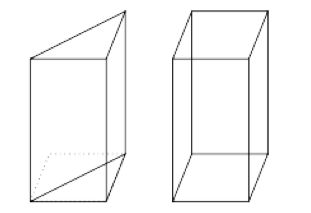
\includegraphics[width=\textwidth ]{../images/sinma2_aiu3_ac80_img01_427488.png}
            \end{minipage}
            \hfill
            \begin{minipage}[b]{0.75\linewidth}
                \begin{oneparchoices}
                    \choice Es igual
                    \choice Es el doble
                    \choice Es la mitad
                    \choice No hay relación
                \end{oneparchoices}
            \end{minipage}
            \part
            \begin{minipage}[b]{0.2\linewidth}
                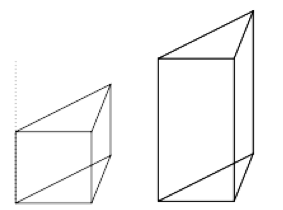
\includegraphics[width=\textwidth ]{../images/sinma2_aiu3_ac80_img02_716612.png}
            \end{minipage}
            \hfill
            \begin{minipage}[b]{0.75\linewidth}
                \begin{oneparchoices}
                    \choice Es igual
                    \choice Es el doble
                    \choice Es la mitad
                    \choice No hay relación
                \end{oneparchoices}
            \end{minipage}
            \part
            \begin{minipage}[b]{0.2\linewidth}
                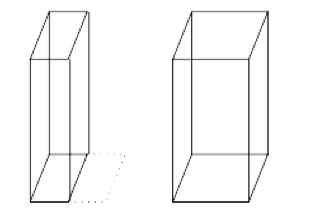
\includegraphics[width=\textwidth ]{../images/sinma2_aiu3_ac80_img03_316634.png}
            \end{minipage}
            \hfill
            \begin{minipage}[b]{0.75\linewidth}
                \begin{oneparchoices}
                    \choice Es igual
                    \choice Es el doble
                    \choice Es la mitad
                    \choice No hay relación
                \end{oneparchoices}
            \end{minipage}
            \part
            \begin{minipage}[b]{0.2\linewidth}
                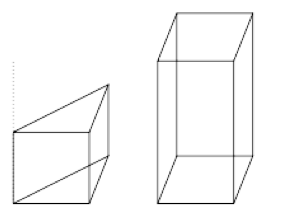
\includegraphics[width=\textwidth ]{../images/sinma2_aiu3_ac80_img04.png}
            \end{minipage}
            \hfill
            \begin{minipage}[b]{0.75\linewidth}
                \begin{oneparchoices}
                    \choice Es el doble
                    \choice Es un cuarto
                    \choice Es la mitad
                    \choice No hay relación
                \end{oneparchoices}
            \end{minipage}
            \part
            \begin{minipage}[b]{0.2\linewidth}
                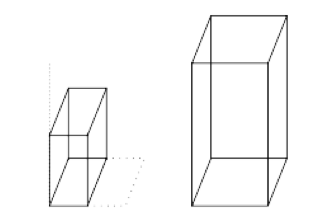
\includegraphics[width=\textwidth ]{../images/sinma2_aiu3_ac80_img05.png}
            \end{minipage}
            \hfill
            \begin{minipage}[b]{0.75\linewidth}
                \begin{oneparchoices}
                    \choice Es el doble
                    \choice Es un cuarto
                    \choice Es la mitad
                    \choice No hay relación
                \end{oneparchoices}
            \end{minipage}
            \part
            \begin{minipage}[b]{0.2\linewidth}
                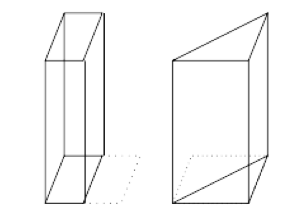
\includegraphics[width=\textwidth ]{../images/sinma2_aiu3_ac80_img06.png}
            \end{minipage}
            \hfill
            \begin{minipage}[b]{0.75\linewidth}
                \begin{oneparchoices}
                    \choice Es el doble
                    \choice Es un cuarto
                    \choice Es la mitad
                    \choice Es igual
                \end{oneparchoices}
            \end{minipage}
            \part
            \begin{minipage}[b]{0.2\linewidth}
                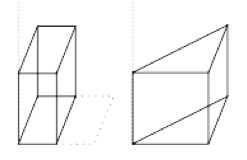
\includegraphics[width=\textwidth ]{../images/sinma2_aiu3_ac80_img07.png}
            \end{minipage}
            \hfill
            \begin{minipage}[b]{0.75\linewidth}
                \begin{oneparchoices}
                    \choice Es igual
                    \choice Es el doble
                    \choice Es la mitad
                    \choice Es un cuarto
                \end{oneparchoices}
            \end{minipage}
        \end{parts}
    }